\chapter{Literature Review} \label{chap:lit-review}
% introduction 
This project aims to facilitate an augmented reality experience, where it could provide suggestions of the classes of objects that can be placed on top of a recognised object in the real-time scene using a Microsoft Kinect Camera. To enable such goal, classification, a form of machine-learning, is proposed to be used in recognising classes of objects in an image. There are many different statistical classification algorithms that can be used for labelling objects through training with similar objects and recognising the category and object belongs when put in use. 

Being an RGB-D camera, not only does the Kinect Camera captures a colour (RGB) image, it also captures depth information via laser combined with a monochrome camera \cite{kinect-doc}. This information enables a detailed 3-dimensional reconstruction. We will look more into the functionality of these cameras.

A group of New York University researchers have created a depth dataset called the \textit{NYU Depth Dataset} \cite{nyu-dataset}, which is freely available online.\footnote{The NYU Depth Dataset V2 is available for download at \url{http://cs.nyu.edu/~silberman/datasets/nyu_depth_v2.html}} A variety of objects are scanned, segmented and labelled from a scene. The variety and the number of scans makes it an ideal candidate as training data for recognising classes of objects with a classification model. We will look into the available datasets in more detail in \autoref{sec:lit-depth-data}.

This Review attempts to explore in greater detail about the NYU Dataset and its applications, how depth maps are useful to 3-dimensional reconstruction and how the depth dataset is useful for training classification models. We will also look at the available algorithms and find out which of them might fit for the task.

\newpage

% Kinect Fusion 
\section{Kinect Fusion}
We start off by looking at Kinect Fusion, where our depth dataset is created from. 

The Kinect Camera was first released for the company's gaming console, XBox 360. It was designed to recognise gestures, faces and voices, providing a more physical way and new dimension to interact with the interface and games than a conventional controller. A Windows-compatible version of the Camera, an SDK and Kinect Fusion were released later, enabling researches and the development of commercial products \cite{kinect-doc}. 

%% FIG - SemanticPaint screenshot
\begin{figure}[h]
  \centering
  \includegraphics[width=0.65\textwidth]{semantic_screen}
  \caption{\textit{A screenshot to show how SemanticPaint utilise depth information from a Kinect camera and Kinect Fusion to colour user-defined areas in real-time. \protect\cite{semantic-paint}}}
  \label{fig:semantic_screen}
\end{figure}

Augmented reality (AR) and real-time reconstructions are some of the most popular research applications of Kinect Fusion. SemanticPaint \cite{semantic-paint} demonstrates the possibility of Kinect Fusion in AR in real-time scenes. It allows parts of the scene to be 'painted' by the user. It also uses segmentation and object recognition to paint similar objects in the same colour. Although this project does not involve real-time processes, it provides the knowledge required to create or use an existing segmentation algorithm for labelling individual items from a scene (discussed later). 

\subsection{Kinect Camera Technologies}
There are two generations of Kinect Camera, where they use different 3-dimensional camera technologies to obtain depth information about a scene. Each of these technologies has its pros and cons, which is discussed below. However, the common problem of these technologies is that it does not deal with very bright light, where detail will be lost \cite{chi-book}. 

\paragraph*{Structured Light}
Structured light is used in the first generation Kinect Camera (2010). A sequence of known infra-red patterns are projected onto the scene. A deformed pattern is formed when objects are 'in the way' of the patterns. The object is then observed from another angle by the monochrome camera. Through analysing the deformed patterns and observations, the depth information about the scene can be obtained \cite{chi-book}\cite{kinect-cam-tech}. It is worth noting that the NYU Dataset \cite{nyu-dataset} uses information captured by the first generation of the Kinect Camera, which is discussed in section \ref{ssec:lit-data_rep}.

\paragraph*{Time-of-Flight}
Rather than looking at the deformed pattern, the second-generation Kinect Camera (2013) estimates depth information based on the time the infra-red or laser beam takes to travel back and forth. The difference between the reference signal and returned signal allows the calculation of a time difference, which helps estimating the required depth information \cite{chi-book}.  

\subsection{Comparing Structured Light and Time-of-Flight}
Structured light cameras obtain more robust depth data than time-of-flight cameras, because it observes the pattern formed rather than being estimated using the time taken for the laser ray to be reflected off the object. 

On the other hand, time-of-flight cameras has more advantages than structure light cameras. For instance, it can handle a much brighter situation - 1W power of light versus 1 $\mu$W \cite{kinect-version-compare}. Also, it is capable of higher frame rate especially when capturing videos, as no software is required to interpret the observed pattern \cite{kinect-cam-tech}.

Although the depth data captured by time-of-flight cameras is less precise, they provide a better real-time experience due to their higher frame rate capability and fewer environmental requirements. 
\\

% FIG - camera tech
\begin{figure}[h]
  \centering
  \includegraphics[width=\textwidth]{camera_tech}
  \caption{\textit{Graphical illustration of the differences between structured light and time-of-flight.}}
  \label{fig:camera_tech}
\end{figure}


\newpage
\subsection{Data Representation} \label{ssec:lit-data_rep}
\subsubsection{Point Cloud and Depth}

%% FIG - Point cloud and depth 
\begin{figure}[ht]
  \centering
  \includegraphics[width=0.7\textwidth]{pt_cloud_depth}
  \caption{\textit{Representing depth in a 3-dimensional space.}}
  \label{fig:pt_cloud_depth}
\end{figure}

A point cloud stores data points in a coordinate system \cite{chi-book}. In a real-world case with captured images, a 3-dimensional space is used. This can be a coordinate system or some other unit such as distances from the camera. In the context of depth from the view of a camera as illustrated in \autoref{fig:pt_cloud_depth}, it can live in some coordinate system which then infer the distance between the formed image and the point in that space. A point cloud can be used to generate a mesh so that it can be used to render a visual image of the reconstruction volume.

\autoref{fig:pt_cloud_depth} also demonstrates the information captured by an RGB-D camera like the Kinect. The image plane shows the normal colour image captured just like any other camera. The 2-dimensional plane is composed of a grid of spots known as pixels, with each representing some form of colours, created using a mixture of different levels of red, green and blue. Depth is the distance between a pixel in the image plane and the actual position of that pixel represents in a real-world, 3-dimensional space.

\subsection{Reconstruction}
\subsubsection{Pipeline}

%% FIG - Kinect Fusion Pipeline
\begin{figure}
  \centering
  \includegraphics[width=0.8\textwidth]{kf_pipeline}
  \caption{\textit{Steps to create a 3D reconstruction with many images. (Taken from \protect\cite{kinect-doc})}}
  \label{fig:k-means}
\end{figure}

A single raw capture with the Camera does not provide much information about a scene. Combining the depth information of many images together enables a super-resolution reconstruction \cite{ms-3d-paper}, creating a detailed and high quality reconstruction. The following is the full pipeline of how a reconstruction is created from raw depth data:
\newpage
\begin{enumerate}
  \item Raw Input Conversion
    \begin{itemize}
      \item The raw \textit{depth map} is captured by the infrared-monochrome subsystem of the Camera. This information is not very detailed. A depth map stores the distance between the RGB image plane and the real world location in a 3-dimensional coordinate system (recall \autoref{fig:pt_cloud_depth}).
      \item It needs to be combined with the \textit{normal map}, which is the surface normals associated with each vertex \cite{szeliski-book}, to provide a more detailed but noisy reconstruction at this stage \cite{kinect-doc}. 
      \item Further conversion and reconstruction is needed to retain detail, remove noise, and fill in holes missed by the Camera, possibly due to bright light.
      \item This information is stored as a point cloud and will be combined into one representation later on.
    \end{itemize}

  \item Camera Pose Tracking
    \begin{itemize}
      \item The location and orientation of each frame, often referred to as the world pose, are tracked as the Camera moves around.
      \item This alignment is constantly traced, allowing all the point clouds to be aligned together \cite{kinect-doc}. 
      \item The frames captured from different poses, even the smallest movement (e.g. caused by a hand-shake), will allow further quality improvements to the scene, achieving more than what a single raw capture is capable of \cite{ms-3d-paper}.
    \end{itemize}

  \item Fusing 
    \begin{itemize}
      \item The depth data converted from the raw input is combined into a single 3-dimensional space per frame.
      \item A running average of depth is kept. This reduces noise, and creates a refined reconstruction by combining all the information in one place \cite{kinect-doc} \cite{ms-3d-paper}. 
    \end{itemize}

  \item Volumetric Integration
    \begin{itemize}
      \item The resultant point cloud will be of a highly detailed reconstruction of the scene. For example, grills of a millimetre \cite{ms-3d-paper} can be reconstructed properly.
      \item A rendered image of the 3D reconstruction volume is possible by using methods such as ray-casting, providing a visual feedback of the scene, and allows for many possibilities, such as augmented reality applications.
    \end{itemize}
\end{enumerate}


\subsubsection{Volumetric Representation}

% FIG - Voxel From External 
%http://www.gamersnexus.net/gg/762-voxels-vs-vertexes-in-games
\begin{figure}[h]
  \centering
  \includegraphics[width=0.65\textwidth]{voxel_ext}
  \caption[caption]{A character represented using a voxel volume\protect\footnotemark}
  \label{fig:voxel_ext}
\end{figure}
\footnotetext{Image taken from \url{http://www.gamersnexus.net/gg/762-voxels-vs-vertexes-in-games}}

By averaging the surface models and depth data from multiple viewpoints into one voxel volume, the scene appears to live in a 3-dimensional 'box' constructed in voxels. As illustrated in \autoref{fig:voxel_ext}, a voxel can be imagined as a 3-dimensional pixel that has some parts 'carved away' to represent the curvatures as perceived in the real world.\cite{szeliski-book}

If this high quality reconstruction can be done fast enough, it can be used for interesting applications, such as an augmented reality experience where virtual particles appear to live and follow the cantor of the scene, as demonstrated by \citeasnoun{ms-3d-paper}. 

\subsection{Segmentation}
In order to perform classification of objects in a scene with many objects, we need to single them out individually so that operations such as labelling can be done. In computer vision, this is called \textit{segmentation}. This is not a simple problem. As illustrated in \autoref{fig:seg-challenge}, segmentation is a subjective task even for human. The image can be segmented in many 'correct' ways.

% FIG - Segmentation Challenges 
\begin{figure}[H]
  \centering
  \includegraphics[width=0.75\textwidth]{seg-challenge}
  \caption{Showing some posibilities of segmentation of one image (Taken from lecture slides created by \protect\citeasnoun{chinery-lec15}).}
  \label{fig:seg-challenge}
\end{figure}

There are much research done on image segmentation. Results produced using unsupervised classifiers such as k-means and mean shift are often used as benchmarks to test against their research (we will discussed about unsupervised classification in \autoref{sec:classification}).

Many approaches have been tried on a wide variety of segmentation problems. For example, \citeasnoun{seg-alpert} uses a probabilistic approach to segment between foreground and background, \citeasnoun{seg-grabcut} utilises both colour and edge information to obtain a 'perfect' foreground image with smoothed edges.

\textbf{Semantic segmentation} is another interesting segmentation problem. It attempts to segment a complex multi-object scene meaningfully. \citeasnoun{nyu-dataset} uses depth information and support inferences to enhance segmentation and labelling of these areas. As a side note, support inferences tells the relationship between objects - e.g., 'if a cup is supported by the book, then the cup must be lifted first' \cite{nyu-dataset}.

More advanced research often introduce new datasets enabling further research. In fact, \citeasnoun{nyu-dataset}'s research resulted in the creation of an extensive depth information dataset known as the \textit{NYU Depth Dataset}. Further research done by \citeasnoun{nyu-improve} improved its labelling accuracy by 20\%. Also, we are going to base our classification dataset on this dataset, which we will now discuss.


\newpage
\section{Depth Data} \label{sec:lit-depth-data}
As the objective of the project is on real-world application, we require a dataset that contains many image scans of a variety of scenes. \citeasnoun{rgbd-datasets} has compiled a list of RGB-D datasets available for research use. Many of the datasets are images of objects in lab setups. While these datasets may enable impressive results more easily, it loses the real-world scenario we are aiming for.

%\textit{TODO: Discuss how Naive Bayes, Decision Trees and SVMs are used in the Forestry Robot paper \cite{forestry}}

\subsection{NYU Depth Dataset V2 \protect\cite{nyu-dataset}}
Quality training data is required to achieve high precision and accuracy. Turns out, the NYU Depth Dataset provides a quality set of depth data which can be used for training a classifier with the aim of achieving high precision and accuracy. There are 1449 densely labelled images from a wide range of scenes in this version. A large, high quality dataset from a wide range of scenarios provide a good base for trying to achieve a high performance model.

% FIG - NYU Dataset Depth image
\begin{figure}[h]
  \centering
  \includegraphics[width=0.95\textwidth]{nyu_depths}
  \caption{\textit{(From left to right) original RGB image, raw depth map, processed depth map (Taken from \protect\citeasnoun{nyu-dataset})}}
  \label{fig:nyu_depths}
\end{figure}

The raw depth information captured by the camera would lose finer, sometimes important, detail. \citeasnoun{nyu-dataset} provides processed depth maps for each of the which contain well-defined objects. The dataset also contains accelerometer metrics (roll, yaw, pitch and tilt) which could be used to normalise the data in these images to point at the same direction.

It also contains labels for each instance of objects in a scene. For example, if there are three chairs, they are labelled as \textit{chair1}, \textit{chair2} and \textit{chair3}. For instance, in computer vision, we might want to match objects between two images so that we can create a panoramic shot (this is beyond the scope of this project).


\newpage

% classifiers
\section{Classification} \label{sec:classification}
The idea of classification is to identify of which group an object belongs to. This relies heavily on a good algorithm that is able to group similar objects together in the first place. In more formal words, a classifier groups objects that has some semantic similarity enough to be classed as the same type. Each class has a label in which these objects are identified as. For example, round objects that can hold liquid can be classed as "bowls", despite being different in colour or and of slightly different shapes \cite{hall-notes}. 


\subsection{Classification Types}
There are many classification models that are fit for different purposes. They are broadly split into two groups - \textit{supervised} and \textit{unsupervised (clustering)}. The following explains what they are and some associated algorithms that could be used as the classifier algorithm for this project.

\subsubsection{Supervised Classification}

% FIG - supervised process
\begin{figure}[h]
  \centering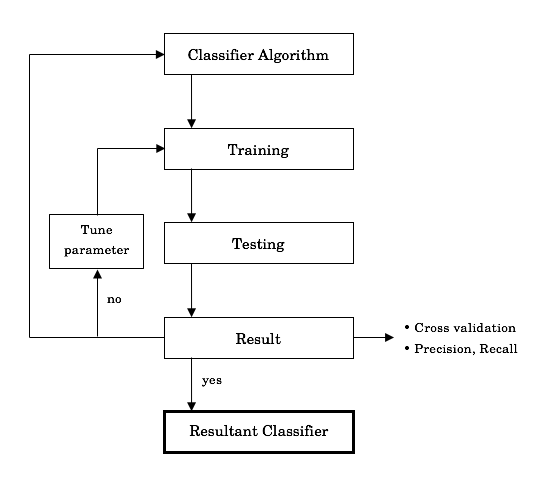
\includegraphics[scale=0.45]{supervised-process.png}
  \caption{An overview of the process for getting a supervised classifier. \protect\cite{class-analysis} }
  \label{fig:supervised-process}
\end{figure}
Supervised learning uses pre-labelled data to train the classifier. Correctly labelled data is given to the classifier at training. This means that the labels and the number of them are pre-defined so that the classifier has a limited amount of choice. The classifier has to aggregate and understand the similarities so to be able to say which class an unknown object is, based on what is already known.~\cite{class-analysis} 

A supervised classifier can either be \textit{probabilistic-based} and \textit{geometric-based}. Probabilistic-based algorithms involves a probabilistic density function (Gaussian distribution being one of the most well-known ones), and are sub-divided into \textit{parametric} and \textit{non-parametric}. For a parametric classifier, the statistical probability distribution of each class is known and is used, whereas the purpose of a non-parametric classifier is to estimate the distribution, as the number of parameters is not known, or does not matter \cite{class-analysis} \cite{hall-notes}.

Supervised learning is ideal when there are an abundance of correctly labelled data for the classifier to learn from. Figure~\ref{fig:supervised-process} describes this graphically. A \textit{training set} contains some pre-labelled data which the classifier algorithm will be trained on. Some of the pre-labelled data is set aside and used as the \textit{test set} to see how well the trained classifier performs. 

We should emphasise the importance of the \textit{test set} to evaluating the performance of a classifier. Overfitting is an issue when the classifier becomes too specific to the training data. In other words, it is treating noise as true signals by taking every minor variation in the training data into account \cite{mur-book}. If a classifier is overfitted by the training data, its ability to predict unseen information is hampered. In such case, we expect a great difference between the training error and testing error. (We see a training accuracy of 50\% versus 1.8\% testing accuracy later in \autoref{chap:results}.) We will further discuss this issue in chapters \ref{chap:tech} and \ref{chap:methodology}. 


\subsubsection{Unsupervised Classification} \label{sssec:unsupervised_overview}
Unsupervised classification is also known as clustering. Items with similar properties in the data level will be grouped together by the algorithm itself. Training is still required, but the label is assigned by the classifier rather than manually. The training data should be unlabelled, to allow the algorithm decide on the number of clusters (labels). Ultimately, the goal with unsupervised learning is to avoid any intervention and let the algorithm do its job \cite{hall-notes}. 

In computer vision, unsupervised classification is mostly used for object recognition in moving scenes and image segmentation. As mentioned, we are going to focus on supervised algorithms to manage the scope of the is project, so that we shall only look briefly into it. 

This should not be confused with \textit{online learning}. Online learning updates the classifier as new datapoints come in \cite{mur-book}. Quality new data should improve the classifier over time. This can be used with both unsupervised and supervised algorithms. For example, a streaming version of random forest is used to learn about newly labelled areas in real-time.


%%%%%%%%%%%%%%%%%%%%%%%%%%%%%%%%%%%%%%%%%
\newpage
\subsection{Classifiers} \label{ssec:classifiers}
We now look at some of popular and notable classification algorithms for both supervised and unsupervised methodologies briefly. We will discuss some of them in detail in \autoref{chap:tech}.

\subsubsection{Notable Supervised Classifiers}
Broadly speaking, there are four groups of supervised classification algorithms, namely, \textit{Bayesian}, \textit{Trees}, \textit{Lazy} and \textit{Functions}. \autoref{tab:supervised-discuss} shows the algorithms and their associated groups that we are going to talk briefly about. 

% TABLE - supervised to be discussed 
\parbox{\linewidth}{
  \centering
  \begin{tabular}{|l|l|}
    \hline
    \multicolumn{1}{|c|}{\textbf{Group}} & \multicolumn{1}{|c|}{\textbf{Model to be discussed}}
    \\\hline
    Bayesian & Naive Bayes (NB) 
    \\\hline
    \multirow{3}{*}{Trees} & Decision tree (DT)
    \\
    & Random forest (RF)
    \\
    & AdaBoost (ADA)
    \\\hline
    Lazy & $K$-nearest neighbours (KNN) 
    \\\hline
    Functions & Support vector machine (SVM)
    \\\hline
  \end{tabular}

  \captionof{table}{\textit{Groups of supervised classification algorithms and their notable examples.}}
  \label{tab:supervised-discuss}
}

\begin{itemize}
  \item \textbf{Naive Bayes (NB)} uses the Bayes' Theorem of probability reasoning (the probability of an event happening given some condition). It also assumes that features are conditionally independent given by Bayes' Theorem, although this may not be true in reality \cite{mur-book}. The algorithm obtains its probability by representing the data as distributions and extracting the class that gives a higher probability. Theoretically, it is robust to overfitting and a simple algorithm.

  \item \textbf{Decision Tree (DT)} is a multiclass classification algorithm that splits the dataset in the input space and gives local models for each region. This creates a tree with each node containing some condition for deciding which children node to go next. By counting the number of datapoints going from the starting node to a leaf for each possible path, we obtain a distribution in the end for each leaf showing the most probable class this path contributes to. This is a simplistic and efficient way in finding different groups within the input space. However, it can be overfitted easily, making it difficult to use with complex datasets. \cite{mur-book}

  \item \textbf{Random Forest (RF)} is an ensemble method. It obtains a prediction by averaging the results of many decision trees, which has proven to be more effective than a single decision tree \cite{compare-supervised}. It attempts to overcome the problem of overfitting by randomising both the features and data used to build each tree.

  \item \textbf{AdaBoost (ADA)} uses boosting to achieve an efficient high quality results (to be discussed in \autoref{sec:boosted}). Over some specified number of iterations, weak learners are trained. A weak learner is one that does not possess much information, but is always be better than random. These weak learners are usually decision trees. 
    
At each iteration, a weight is added to misclassified datapoints, which is then used by the next iteration to train the next weak classifier. Additively, the resultant classifier becomes a robust classifier that provides strong classification power \cite{boosting}.

  \item \textbf{$K$-Nearest Neighbours (KNN)} uses $K$ datapoints around each datapoint to obtain the class it belongs to. Despite being a non-parametric model means that it is fast to train, it assumes strongly about the data distribution, as each datapoint simply takes the count of each class in the surrounding datapoints to decide on its class. Other downsides include complex decision boundaries and does not work well with high dimensional datasets due to the curse of dimensionality \cite{mur-book}. 

  \item \textbf{Support Vector Machines (SVM)} aims to maximise the margins which runs parallel to the decision boundary and are defined by points of each class. It is a popular algorithm because of its versatility, with many tunable parameters and kernels for different distributions of data. It started off being a binary classifier, but is extended for multiclass classification by building multiple classifiers and comparing between them \cite{bishop-book}. 
\end{itemize}

\textit{Note that from now on, we will use the acronyms stated next to the aforementioned alogirthms for clarity. For instance, we will refer to Support Vector Machine as SVM.}
\\

% TABLE - comparison
\parbox{\linewidth}{
  \centering
  \begin{tabular}{|c|c|c|c|}
    \hline
    \textbf{Model} & \textbf{Training Speed} & \textbf{Classification Speed} & \textbf{Mean Accuracy}
    \\\hline
    BST-DT   & Fast           & Fast        & 89.6\%
    \\\hline
    RF       & Rather fast    & Rather fast & 89.2\%
    \\\hline
    SVM      & Slowest        & Slowest     & 86.2\%
    \\\hline
    KNN      & Rather fast    & Rather fast & 81.5\%
    \\\hline
    DT       & Very fast      & Very fast   & 70.9\%
    \\\hline
    NB       & Fastest        & Fastest     & 65.4\% 
    \\\hline
  \end{tabular}

  \captionof{table}{\textit{Comparing properties of different classification models (adapted from \protect\citeasnoun{compare-supervised})}}
  \label{tab:comparison}
}

\citeasnoun{compare-supervised} performed 11 tests on widely available benchmark datasets on many supervised classifiers. \autoref{tab:comparison} shows the properties of some of these classifiers and their average results on these 11 tests. Note that this can only be used as a benchmark as our dataset will be much more complicated and large than the ones used in their paper. 

Tests done by \citeasnoun{compare-supervised-2} and the descriptions in the \texttt{scikit-learn} documentation (we will discuss more about \texttt{scikit-learn} in \autoref{sec:lit-tools}). Both suggest that SVM can outperform Random Forest with proper parameter tuning and kernel settings, but the trade-off is speed.

SVM is known to not scale well and could require a long training time compared to other models \cite{compare-supervised}. However, it is also one of the popular machine-learning algorithms used for classification and regression problems, due to its ability to be customised with parameters and different kernels to cater for different shapes and density of the input data. We shall discuss more about this in \autoref{sec:tech-SVM}.

Tree methods (Boosted Decision Tree (BST-DT), DT and RF) and SVM have different algorithms underneath. Tree methods obtain their good performance through an appropriate amount of randomisation of the training dataset, whereas SVM does so by choosing the right kernel and tweaking its parameters. In \autoref{chap:tech}, we shall discuss in depth their properties.

Despite KNN seems to perform relatively well compared to DT and NB, our dataset will be highly dimension (discussed in \autoref{chap:methodology}), meaning that it would not be the best choice of classifier in our case. And, we could most likely disregard DT and NB due to their relatively poor accuracy even with benchmark data.

This leaves us with BST-DT, RF and SVM. In fact, they are widely used to solve classification problems. For instance, \cite{semantic-paint} uses an online learning varient of RF to train newly labelled items so to paint that class of objects in the scene with the same colour. In \autoref{chap:results}, we are going to find out if these algorithms produce respectable results.


\subsubsection{Notable Unsupervised Classifiers}
As mentioned in the introduction, we are going to focus on supervised classification to limit the scope of this project. Nonetheless, we should briefly look at some popular unsupervised algorithms. In fact, we will be using $K$-means clustering for a different reason than training a classifier or image segmentation, but to engineer our dataset. We will discuss this in \autoref{chap:methodology}.

Unsupervised classification models are also known as \textit{clustering}. It aims to group similar objects together \cite{mur-book}. Broadly speaking, we can split clustering algorithms into three categories, namely, \textit{centroid-based}, \textit{distribution-based} and \textit{density-based}. Let us discuss about the models mentioned in \autoref{tab:unsupervised-discuss}.

% TABLE - supervised to be discussed 
\parbox{\linewidth}{
  \centering
  \begin{tabularx}{0.8\textwidth}{|l|X|}
    \hline
    \multicolumn{1}{|c|}{\textbf{Group}} & \multicolumn{1}{c|}{\textbf{Model to be discussed}}
    \\\hline
    Centroid-based & $K$-means 
    \\\hline
    Distribution-based & Gaussian Mixture Models with Expectation Maximisation (GMM with EM)
    \\\hline
    Density-based & DBSCAN
    \\\hline
  \end{tabularx}

  \captionof{table}{\textit{Groups of unsupervised classification algorithms and their notable examples.}}
  \label{tab:unsupervised-discuss}
}

\begin{itemize}

  \item \textbf{$K$-means clustering} takes $K$ random datapoints to be the starting point. These points are moved until the groups become stable and produces groups with minimal distances between each point and their surroundings. These points would end up being the mean of their corresponding cluster ($\mu_k$ for a cluster $k$), also known as centroids \cite{bishop-book}.

  \item \textbf{Gaussian mixture model} combines multiple Gaussian distributions by imposing them to capture more information about the dataset \cite{bishop-book}. Similar to $K$-means, each Gaussian $k$ centres around the mean $\mu_k$, but also introduces covariance to allow it to work with high dimensionality in the data. However, the amount of tunable parameters make it rather unscalable \cite{scikit-docs}.

Finding parameters are simple when complete data is available, but usually not the case. With the help of the Expectation Maximisation algorithm (often referred to the EM algorithm), it iteratively finds missing values by fixing some parameters (the E step), and then optimising the parameters with these new values (the M step) \cite{mur-book}. In fact, this method can be applied to many clustering models, including $K$-means. We will see this more formally in \autoref{sec:tech-kmeans}.

  \item \textbf{DBSCAN} is a model that finds clusters of any shape by separating out high density as clusters, but spiral datasets in particular. It looks at how many neighbouring points there are in its surrounding to decide if it belongs to a particular cluster. This is effective in distinguishing between noise and cluster membership, but not in locating closed-by clusters \textit{DBSCAN}. It is even more autonomous in the sense that it does not required a specified number of clusters like $K$-means.
\end{itemize}


%%%%%%%%%%%%%%%%%%%%%%%%%%%%%%%%%%%%%%%%%
\section{Performance}
After we trained a classifier, we have to evaluate its performance. As mentioned in the Introduction, we can use various methods to find this out. In this section, we will look into precision-recall rates and the confusion matrix. 

\subsection{Precision and Recall}
The precision and recall rates (accuracy) can be calculated to analyse the performance of the classifier \cite{precision-recall}. They are calculated by comparing predictions against the actual values.

\parbox{\linewidth} {
  \centering
  \begin{tabular}{|l|c|c|}
    \hline
                        & Actual Positive & Actual Negative
    \\ \hline
    Predicted Positive  & TP              & FP
    \\ \hline
    Predicted Negative  & FN              & TN
    \\ \hline
  \end{tabular}

  \captionof{table}{Confusion matrix (taken from \protect\citeasnoun{precision-recall})}
  \label{tab:cm}
}

In order to calculate these rates, a confusion matrix is computed. It is a table that puts the correctness of predictions against the actual values of the underlying data (Table~\ref{tab:cm}). This shows the number of correct and incorrect recognition, allowing a couple of metrics to be calculated, notably precision and recall. (Table~\ref{tab:eq}) 

\parbox{\linewidth} {
  \centering
  \begin{tabular}{|l|}
    \hline \\
    \( \text{Recall}              = \frac{TP}{TP + FN} \) \\[10pt]
    \( \text{Precision}           = \frac{TP}{TP + FP} \) \\[10pt]
    \( \text{True Positive Rate}  = \frac{TP}{TP + FN} \) \\[10pt]
    \( \text{False Positive Rate} = \frac{FP}{FP + TN} \) \\~\\
    \hline
  \end{tabular}
  
  \captionof{table}{\textit{Common machine-learning evaluation metrics (taken from~\protect\citeasnoun{precision-recall}).}}
  \label{tab:eq}
}

Precision and recall takes into account all the true-false positives and negatives. Precision is the positive predictive value -- \textit{``how many selected items are relevant''}, whereas recall explains the sensitivity -- \textit{``how many relevant items are selected''}, as seen in \autoref{tab:eq} and \autoref{fig:precision_recall}. The former tells us how well the model can predict correctly; the latter tells us the \textit{quantity} of which the relevant items is picked \cite{precision-recall-wiki}.

To say that a model is \textit{good for use}, it has to be both precise and has a high recall rate. If a model is very precise, but does not pick up much of the relevant items, the model might look as if it was performing well, but in fact, it has hardly picked out enough of the right items; vice versa.

% FIG: precision recall
\begin{figure}[H]
  \centering
  \includegraphics[width=0.65\textwidth]{precision_recall}
  \caption{\textit{ Diagram representation of precision and recall (adapted from \protect\citeasnoun{precision-recall-wiki}). }}
  \label{fig:precision_recall}
\end{figure}

\subsection{Cross-validation}
It is important to ensure that the training and testing sets are different and that there is no overlap between the two sets, otherwise overfitting will happen. Overfitting is evident when a classifier appears to be functioning perfectly during the train-and-test stage, but turns out to be unable to classify new objects when put into use. On top of the training and test sets, a third validation subset can be introduced. This enables an extra check to ensure that the classifier actually works.  However, the precision and accuracy of the classifier could suffer as a result of a smaller training set \cite{cross-val-scikit}. 

Cross-validation solves the problem by creating some \textit{mutually exclusive} folds (subsets). These folds are created after a test set is taken out from the original set of data. One popular algorithm is $k$-fold cross-validation. It does not run validation on all possible splits on the folds but one different split for each run to save on computational complexity. Multiple cross-validation runs with different splits are performed, resulting in an average that estimates the complete cross-validation \cite{cross-val-kohavi}. This gives an unbiased view as to how the classifier performs, as it is not limited to one fixed set of testing data.

\subsection{Evaluating Unsupervised Classifier}
Although we are not attempting clustering as a classification solution, we should understand the methods that can be used to evaluate them.

Clustering methods are more difficult to evaluate, but not dissimilar to how supervised classifiers are evaluated \cite{mur-book}. There are two types of evaluations. \textit{Internal evaluation } looks at the data from within the cluster, much like the training accuracy in a supervised classifier in which we try to predict the same set of data as used for training it. \textit{External evaluation} uses data that has not been seen before, which is similar to evaluations of supervised classifier that obtain a test set accuracy value.

% TABLE - supervised to be discussed 
\parbox{\linewidth}{
  \centering
  \begin{tabular}{|l|l|}
    \hline
    \multicolumn{1}{|c|}{\textbf{Type}} & \multicolumn{1}{c|}{\textbf{Method}}
    \\\hline
    \multirow{3}{*}{Internal Evaluation} & Davies-Bouldin Index
    \\ & Dunn Index
    \\ & Silhouette Coefficient
    \\\hline
    \multirow{5}{*}{External Evaluation} & Rand Measure
    \\ & F-measure (F-score)
    \\ & Jaccard Index
    \\ & Fowlkes-Mallows Index
    \\ & Mutual Information
    \\ & Confusion Matrix
    \\\hline
  \end{tabular}

  \captionof{table}{\textit{Evaluation methods for unsupervised classifiers (clustering).}}
  \label{tab:unsupervised-eval}
}

Internal methods aim to evaluate the separation and density between clusters, and identifying outlying points. Most external methods require a ground-truth dataset (an unseen labelled dataset that can be used to compare with the trained model) \cite{cluster-label}. For instance, F-measure provides a single value by taking the mean of precision and recall harmoniously. 

%%%%%%%%%%%%%%%%%%%%%%%%%%%%%%%%%%%%%%%%%
\newpage
\section{Tools for Machine-learning Application} \label{sec:lit-tools}
There are many tools out there that provides machine-learning capabilities. For the purpose of this project, we are going to use Python due to the availability of some useful packages and our familiarity of the language. 

Nevertheless, we shall look into the three most popular languages and their associated libraries for machine-learning. 

\subsection{Python}
Python is a general purpose programming languages widely used for scripting tasks. It is one of the top programming languages used for many purposes. It provides a wide range of libraries for different tasks. Python is open-sourced, meaning that it is freely available for use. However, Python suffers from Global Interpreter Lock, disallowing multiple threads to run at one time \cite{gil}. This could hamper performance when a large amount of memory or parallelism is required.

\begin{itemize}
  \item \texttt{scikit-learn} is an actively developed machine-learning library for Python. It has quality implementations of popular machine-learning algorithms for different machine-learning problems. It is built on \texttt{numpy} and \texttt{scipy}, making it easy for data manipulation \cite{scikit-learn-paper}. 
    
A wide range of companies and researches use scikit learn for machine-learning purposes, including Spotify and Evernote.\footnote{According to scikit-learn at \url{http://scikit-learn.org/stable/testimonials/testimonials.html}.} \citeasnoun{scikit-learn-paper} compared it with other Python machine-learning packages which sees scikit-learn beating the others in baseline tests. It provides implementations of the supervised and unsupervised classification algorithms implementations we briefly mentioned in section \ref{ssec:classifiers}.

  \item \texttt{numpy} is a powerful tool for manipulating and storing arrays. It allows an array to be reshaped into any dimension without altering the underlying data. Its powerful memory management enables this, and is able to be represented much more efficiently than the built-in list structures of Python \cite{numpy}.
\end{itemize}

\subsection{R}
\texttt{R} is a popular language used by the data analytics and data science community. It provides an extensive selection of libraries for data manipulation and machine-learning purposes. It provides great visiualisation libraries such as \texttt{ggplot2} for graph plotting and \texttt{data.tables} for efficient data manipulation.

R is an open-sourced statistical programming language. It has an engaged community and can be used in conjunction with other popular general-purpose programming languages.Also, R has a large presence big technology companies, such as Google, Facebook and Twitter, as well as in academia and sciences. \footnotemark  However, R has a steep learning curve because of its syntax. And, it is known to not scale very well as data has to be stored on RAM and can only be run in a single thread.

\footnotetext{According to Revolution Analytics, maker of R, at \url{http://www.revolutionanalytics.com/companies-using-r}.}

\subsection{MatLab}
MatLab is widely used mainly in academia, and research and development purposes. It provides quick prototyping due to its high-level language. It also contains many libraries and toolbox to perform a wide range of operations. For instance, the Image Processing Toolbox provides for computer vision application, such as image filtering which is used for edge detection. For classification, MatLab has implementations for popular algorithms that we mentioned previously.

\subsection{Choosing a Tool}
It is difficult to decide which language is the best. Like any programming situation, there is no one language that is superior than another. There is only one that is more suitable than another based on its capability to perform the said task.

In this case, they all provide rich libraries and community support with many guides available. R and Python are the languages used by the popular data science competition website, \href{http://www.kaggle.com}{Kaggle}, while MatLab is well-established in academia with an abundance of libraries, making it a difficult decision.

Python is chosen because of its simple syntax and our personal experience with it. It is shown to have solved real-life machine-learning problems for reputable companies and widely used. Also, being a language that is widely used for scripting purposes, command line arguments can be used to supply variables to the underlying code without having to change the code itself. This is particularly useful for this project, as we would have to 

\section{Hardware Considerations}
We are potentially dealing with many datapoints of large feature vectors. Although a moderately modern computer with relatively large amount of memory and multi-core processors will suffice to moderately challenging machine-learning tasks, it would be ideal to be able to off-lift these heavy operations to a more powerful system that we could use any time anywhere with an Internet connection.

There are two notable options - the High Performance Computer cluster at the University, Balena\footnote{https://wiki.bath.ac.uk/display/BalenaHPC/Balena+High+Performance+Computing+Service}, and Amazon EC2\footnote{https://aws.amazon.com/ec2/}. They are both ideal services as they provide flexibility and scalability that cannot be matched by a personal laptop. The following discusses some of their features, and pros and cons.

\begin{itemize}
  \item \textbf{Balena} \\ \\
    It is made up of many computers to form one big connected computer service. It contains 88 nodes of 64GB of memory and 80 nodes of 128GB of memory. A user can submit a job with a simple script and it will enter a queue. The job will run when appropriate resource is available and that the job has reached the top of the queue. Also, it supports parallel computing, where multiple node can be used together to perform some tasks. This service can be accessed by any University of Bath personnel that has a use-case for it. 
    
    There are different groups of accounts available. For a free account, a user can only run jobs up to 6 hours and has limits on how many computing-hours that one can be used at one time. Also, there may be long queue times at busy periods when the cluster has a high-volume of jobs. 
  \\ 
  \item \textbf{Amazon EC2} \\ \\
    Amazon EC2 (Elastic Compute Cloud) has been the computing platform used by many renowned companies such as Airbnb and Netflix. It is a very flexible system in that a user can start a new instance of their preferred distribution of Linux Microsoft Windows Server quickly, with various processor and memory configurations. The user assumes complete control of the system. It acts as a real machine so that they can install and configure the system as it suits them. 
    
    However, there is much overhead to get the instance ready to perform the required tasks for this project. For instance, it might be required to install the appropriate packages and libraries every time we start up a new instance, before any task can take place. Also, it gets quite expensive when more memory is required, as it is charged per hour for when the instance is running. And, there is not the luxury of running many jobs over multiple machines to perform parallel operations.
\end{itemize}

Given access to a free service providing great computing resource, Balena is the obvious choice. Although there is a time limit and queue times may vary during the course of this project, it provides a great platform to run large code without much overhead in setting up the servers before they can be used. On the other hand, while AWS provides complete control about the system and has great flexibility, the cost of running a decent server could go up quickly as more memory and computing time is required.


%%%%%%%%%%%%%%%%%%%%%%%%%%%%%%%%%%%%%%%%%
% summary
\newpage
\section{The Project}
In this chapter, we learnt about that depth information can be useful for different applications. We also looked at the NYU Depth Dataset to find that it contains useful information which could be used as our base dataset.

We examined different classification algorithms and found out that BST-DT, RF and SVM perform the best in benchmark comparisons. There are a few algorithms for performing boosting with decision trees. We are going to use AdaBoost as it is one of the most regarded implementations of boosting (discussed in detail in \autoref{sec:tech-boosted}. We are going to see how they perform with our dataset in \autoref{chap:results}. After all, no one classification method fits all problem. It is not known how well perform or whether they will fit for the purpose at all.

After we have trained some classifiers, it is important to conduct many tests to ensure it is performing properly and well. As discussed, precision-recall rates and cross-validation are helpful tools to evaluate the performance of the classifiers. They should be performed the classifier performs properly by examining it with data. Also, recall that a \textit{test dataset} for testing purposes to find out the predictive power of a classifier. If there is a huge difference between training and test dataset error, it is an evidence of overfitting.

As for tools, we decided to use Python and its associated libraries due to our familiarity with the language and its popularity for machine learning. 

Also, we decided to use Balena as our computer resource to perform machine-learning tasks, as it has much more processing power and memory than an ordinary laptop. However, we have to take into account the limitations as a free user on Balena. 

Now that we have established a background knowledge about the problem space and the tool to use, we will look into detail of how our chosen classifiers work formally next.
